%%%%%%%%%%%%%%%%%%%%%%%%%%%%%%%%%%%%%%%%%
% Masters/Doctoral Thesis 
% LaTeX Template
% Version 1.43 (17/5/14)
%
% This template has been downloaded from:
% http://www.LaTeXTemplates.com
%
% Original authors:
% Steven Gunn 
% http://users.ecs.soton.ac.uk/srg/softwaretools/document/templates/
% and
% Sunil Patel
% http://www.sunilpatel.co.uk/thesis-template/
%
% License:
% CC BY-NC-SA 3.0 (http://creativecommons.org/licenses/by-nc-sa/3.0/)
%
% Note:
% Make sure to edit document variables in the Thesis.cls file
%
%%%%%%%%%%%%%%%%%%%%%%%%%%%%%%%%%%%%%%%%%

%----------------------------------------------------------------------------------------
%   PACKAGES AND OTHER DOCUMENT CONFIGURATIONS
%----------------------------------------------------------------------------------------

\documentclass[11pt, oneside]{Thesis} % The default font size and one-sided printing (no margin offsets)

\graphicspath{{figs/}} % Specifies the directory where pictures are stored

\usepackage[square, numbers, comma, sort&compress]{natbib} % Use the natbib reference package - read up on this to edit the reference style; if you want text (e.g. Smith et al., 2012) for the in-text references (instead of numbers), remove 'numbers' 
\usepackage{amsmath}
\usepackage{booktabs}
\usepackage{cancel}
\usepackage{caption}
\usepackage{cleveref}
\usepackage{colortbl}
\usepackage{csquotes}
\usepackage{helvet}
\usepackage{mathpazo}
\usepackage{multirow}
\usepackage{listings}
\usepackage{pgfplots}
\usepackage{xcolor}
\usepackage{siunitx}

\hypersetup{urlcolor=blue, colorlinks=true} % Colors hyperlinks in blue - change to black if annoying
\title{\ttitle} % Defines the thesis title - don't touch this

\begin{document}

\frontmatter % Use roman page numbering style (i, ii, iii, iv...) for the pre-content pages

\setstretch{1.3} % Line spacing of 1.3

% Define the page headers using the FancyHdr package and set up for one-sided printing
\fancyhead{} % Clears all page headers and footers
\rhead{\thepage} % Sets the right side header to show the page number
\lhead{} % Clears the left side page header

\pagestyle{fancy} % Finally, use the "fancy" page style to implement the FancyHdr headers

\newcommand{\HRule}{\rule{\linewidth}{0.5mm}} % New command to make the lines in the title page

%% marc's commands
\newcommand{\pt}{p$_{\text{T}}$ }

%energies
\newcommand{\mev}{\si{\mega\electronvolt}}
\newcommand{\gev}{\si{\giga\electronvolt}}
\newcommand{\tev}{\si{\tera\electronvolt}}

%distances
\newcommand{\nm}{\si{\nano\meter}}
\newcommand{\mm}{\si{\milli\meter}}
\newcommand{\cm}{\si{\centi\meter}}

% PDF meta-data
\hypersetup{pdftitle={\ttitle}}
\hypersetup{pdfsubject=\subjectname}
\hypersetup{pdfauthor=\authornames}
\hypersetup{pdfkeywords=\keywordnames}

%----------------------------------------------------------------------------------------
%   TITLE PAGE
%----------------------------------------------------------------------------------------

\begin{titlepage}
\begin{center}

\textsc{\LARGE \univname}\\[1.5cm] % University name
\textsc{\Large Doctoral Thesis}\\[0.5cm] % Thesis type

\HRule \\[0.4cm] % Horizontal line
{\huge \bfseries \ttitle}\\[0.4cm] % Thesis title
\HRule \\[1.5cm] % Horizontal line
 
\begin{minipage}{0.4\textwidth}
\begin{flushleft} \large
\emph{Author:}\\
\href{http://www.johnsmith.com}{\authornames} % Author name - remove the \href bracket to remove the link
\end{flushleft}
\end{minipage}
\begin{minipage}{0.4\textwidth}
\begin{flushright} \large
\emph{Supervisor:} \\
\href{http://www.jamessmith.com}{\supname} % Supervisor name - remove the \href bracket to remove the link  
\end{flushright}
\end{minipage}\\[3cm]
 
\large \textit{A thesis submitted in fulfilment of the requirements\\ for the degree of \degreename}\\[0.3cm] % University requirement text
\textit{in the}\\[0.4cm]
\groupname\\\deptname\\[2cm] % Research group name and department name
 
{\large \today}\\[4cm] % Date
%\includegraphics{Logo} % University/department logo - uncomment to place it
 
\vfill
\end{center}

\end{titlepage}

%----------------------------------------------------------------------------------------
%   DECLARATION PAGE
%   Your institution may give you a different text to place here
%----------------------------------------------------------------------------------------

\Declaration{

\addtocontents{toc}{\vspace{1em}} % Add a gap in the Contents, for aesthetics

I, \authornames, declare that this thesis titled, '\ttitle' and the work presented in it are my own. I confirm that:

\begin{itemize} 
\item[\tiny{$\blacksquare$}] This work was done wholly or mainly while in candidature for a research degree at this University.
\item[\tiny{$\blacksquare$}] Where any part of this thesis has previously been submitted for a degree or any other qualification at this University or any other institution, this has been clearly stated.
\item[\tiny{$\blacksquare$}] Where I have consulted the published work of others, this is always clearly attributed.
\item[\tiny{$\blacksquare$}] Where I have quoted from the work of others, the source is always given. With the exception of such quotations, this thesis is entirely my own work.
\item[\tiny{$\blacksquare$}] I have acknowledged all main sources of help.
\item[\tiny{$\blacksquare$}] Where the thesis is based on work done by myself jointly with others, I have made clear exactly what was done by others and what I have contributed myself.\\
\end{itemize}
 
Signed:\\
\rule[1em]{25em}{0.5pt} % This prints a line for the signature
 
Date:\\
\rule[1em]{25em}{0.5pt} % This prints a line to write the date
}

\clearpage % Start a new page

%----------------------------------------------------------------------------------------
%   QUOTATION PAGE
%----------------------------------------------------------------------------------------

\pagestyle{empty} % No headers or footers for the following pages

\null\vfill % Add some space to move the quote down the page a bit

\textit{``Thanks to my solid academic training, today I can write hundreds of words on virtually any topic without possessing a shred of information, which is how I got a good job in journalism."}

\begin{flushright}
Dave Barry
\end{flushright}

\vfill\vfill\vfill\vfill\vfill\vfill\null % Add some space at the bottom to position the quote just right

\clearpage % Start a new page

%----------------------------------------------------------------------------------------
%   ABSTRACT PAGE
%----------------------------------------------------------------------------------------

\addtotoc{Abstract} % Add the "Abstract" page entry to the Contents

\abstract{\addtocontents{toc}{\vspace{1em}} % Add a gap in the Contents, for aesthetics

The Thesis Abstract is written here (and usually kept to just this page). The page is kept centered vertically so can expand into the blank space above the title too\ldots
}

\clearpage % Start a new page

%----------------------------------------------------------------------------------------
%   ACKNOWLEDGEMENTS
%----------------------------------------------------------------------------------------

\setstretch{1.3} % Reset the line-spacing to 1.3 for body text (if it has changed)

\acknowledgements{\addtocontents{toc}{\vspace{1em}} % Add a gap in the Contents, for aesthetics

The acknowledgements and the people to thank go here, don't forget to include your project advisor\ldots
}
\clearpage % Start a new page

%----------------------------------------------------------------------------------------
%   DEDICATION
%----------------------------------------------------------------------------------------

\setstretch{1.3} % Return the line spacing back to 1.3

\pagestyle{empty} % Page style needs to be empty for this page

\dedicatory{For/Dedicated to/To my\ldots} % Dedication text

\addtocontents{toc}{\vspace{2em}} % Add a gap in the Contents, for aesthetics

%----------------------------------------------------------------------------------------
%   Table of contents
%----------------------------------------------------------------------------------------
\pagestyle{fancy}

\lhead{\emph{Contents}} % Set the left side page header to "Contents"
\tableofcontents % Write out the Table of Contents

%----------------------------------------------------------------------------------------
%   THESIS CONTENT - CHAPTERS
%----------------------------------------------------------------------------------------

\mainmatter % Begin numeric (1,2,3...) page numbering

\pagestyle{fancy} % Return the page headers back to the "fancy" style

% Include the chapters of the thesis as separate files from the Chapters folder
% Uncomment the lines as you write the chapters

% Some commands used in this file
\newcommand{\package}{\emph}

\chapter{Introduction}

The construction of the LHC and its experiments over the few last decades has been only
the last step in a long and successful history of particle accelerators that started roughly 100 years
ago with the construction of the first 



\section{Features}
\label{sec:features}





\chapter{Theory}
\label{ch:theory}
In order to interpret any experimental result, it is of paramount importance to understand
the underlying model governing the physical processes in question. Modern physics knows a
large number of rather successful theories all dedicated to describing different mass and 
energy scales. An example is the theory of classical mechanics, which manages to describe the 
physics of `daily life' very well. However, it breaks down when velocities approach
the speed of light and has to be incorporated into a broader theory, namely that of relativity.

This specific example already suggests that different physical theories are valid only in a 
certain energy range and describe only a certain `type'\footnote{In this particular example
electromagnetic interactions are -- for instance -- not described at all.} of physical process. 
This fact is also true for the case of particle physics. The relevant theory is called the 
\textit{`Standard Model'} and will be described hereafter. Further into the chapter,
a short description of the pitfalls of the standard model will be given with some explanation
on possible solutions.

\section{The Standard Model}
\label{sec:standardmodel}
The Standard Model (SM) of particle physics provides the theoretical framework that
describes all fundamental particles and the forces that act between them, with the one
exception of gravity. Despite a few drawbacks that will be described later (see Section~\ref{sub:sm_shorts})
it has been an overwhelmingly successful theory, capable of describing experimental data
with a precision that is simply outstanding.

\subsection{Particle content in the Standard Model}
\label{sub:sm_particles}
\subsection{Shortcomings of the Standard Model}
\label{sub:sm_shorts}
\section{Supersymmetry}
\label{sec:susy}
\subsection{Particle content}
\label{sub:susy_particles}
\subsection{Observables for searches for Supersymmetry}
\label{sub:susy_observables}
\section{Remaining open questions in particle physics}
\label{sec:theory_remains}

\chapter{Experimental Setup}
\label{ch:exp}

All data analysed in this thesis was recorded with the CMS experiment at the Large Hadron
Collider (LHC) at the European Organization for Nuclear Research (CERN) near Geneva, Switzerland.
This chapter provides a short overview of CERN and its accelerators, the LHC, as well as a
short description of the main components of the CMS experiment.

\section{The Large Hadron Collider}
\label{sec:lhc}
The LHC \cite{lhc_designreport} is currently by far the largest and most powerful particle accelerator in
the world. It is a circular accelerator situated in a tunnel around 100 metres below the Swiss-French
border west of Geneva. Its main purpose is accelerating protons to energies of up to 13 TeV
\footnote{One electronvolt (eV) is the energy acquired by a charge of 1$e$ passing through an electric field of 1 volt, equivalent to \num{1.602e-19} Joule.} 
in the final development stage of the machine starting in 2015. 
Besides the acceleration of protons it is also capable of accelerating heavy ions (predominantly lead ions) to energies of up to 
2.76 TeV per nucleon.

\subsection{The acceleration chain}
\label{sub:chain}
Particles injected into the LHC for final acceleration are required to have an energy of 450 GeV. This is
achieved by a long chain of linear and circular accelerators, a sketch of which can be seen in
Fig.~\ref{fig:accelerators}. 

\begin{figure}[h!]
    \centering
    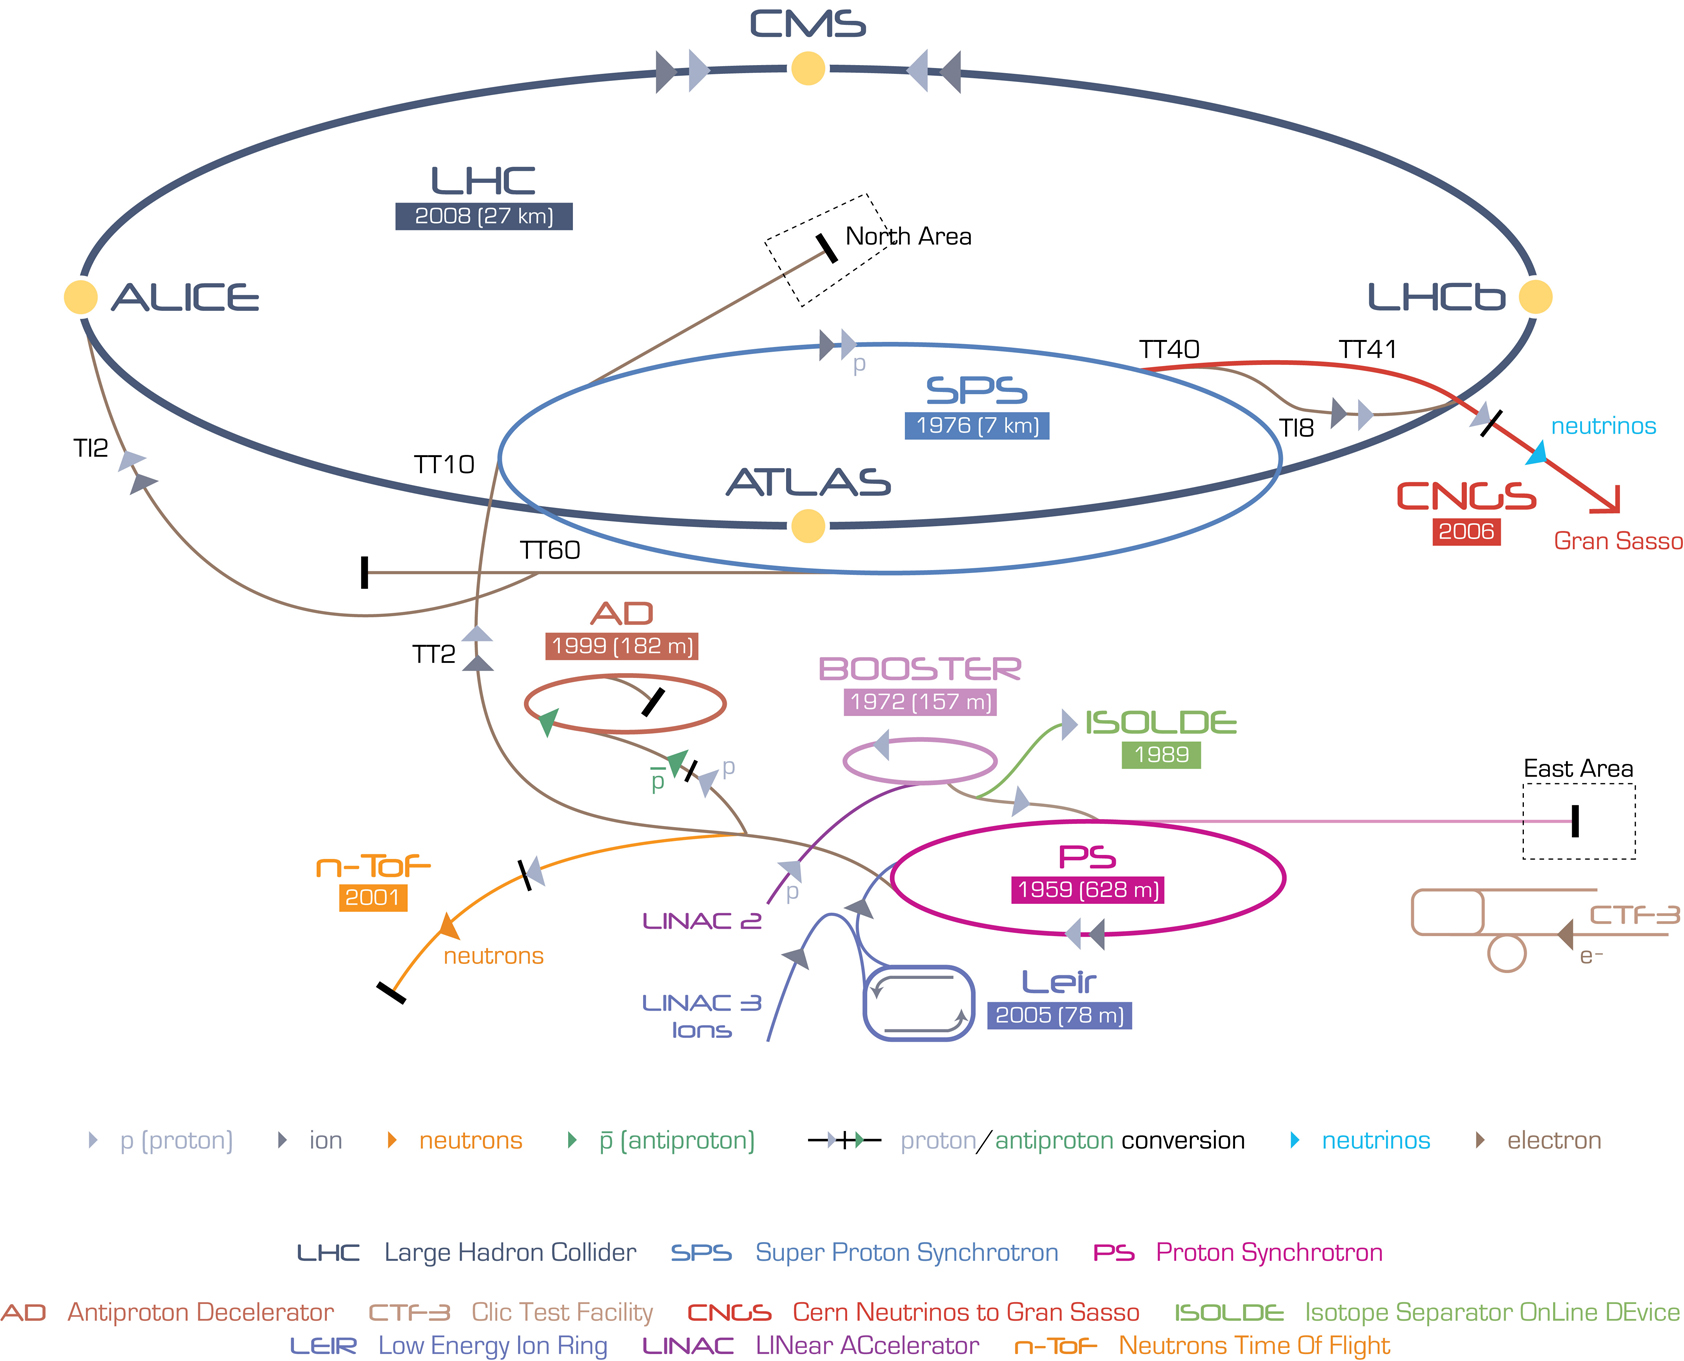
\includegraphics[width=0.65\textwidth]{../figs/Cern-Accelerator-Complex.jpg}
    \caption{Conceptual drawing of all accelerators and experiments hosted at CERN. Besides operating
    the LHC, there are many other accelerators, decelerators and experiments being operated.}
    \label{fig:accelerators}
\end{figure}

Protons used for acceleration in the LHC are extracted from a hydrogen molecules in a bottle situated 
at the CERN main site. These molecules are stripped of their electrons by strong electric fields
and subsequently injected into the first acceleration stage, the linear accelerator Linac 2. Upon exiting
Linac 2, the protons have gained an energy of 50 MeV and are injected into the first circular accelerator,
the Booster. This synchrotron with a circumference of 157 meters accelerates the protons to an energy of 1.4 GeV and
uses magnetic dipole fields to bend the protons onto a circular path. These bending magnets are operated at 
room temperature for the Booster and in fact all the accelerators up to the LHC.
From the Booster, the protons are injected further into the Proton Synchrotron, an accelerator originally built
in 1959 with a circumference of 628 meters and an output energy of 25 GeV. The last step before injection into
the LHC is the Super Proton Synchrotron (SPS), which accelerates the protons to the LHC injection energy of 450 GeV.
The SPS is the world's second largest accelerator with a circumference of nearly 7 km, and it was the first accelerator
to collide protons and anti-protons at energies high enough to produce $W$ and $Z$ bosons, leading to their discovery in 1983
\cite{Wdiscovery, Zdiscovery}.

Ions pass through the same accelerators on their way to the LHC, the only difference being the
first linear accelerator, which in the case of heavy ions is Linac 3.

While the LHC is filled and delivering collisions to its experiments, the accelerators are used to provide
particles to other experiments ongoing at CERN. The Antiproton Decelerator (AD) in which anti-protons are 
decelerated and combined with positrons to form anti-hydrogen, and the ISOLDE collaboration for the study
of many different radioactive ions are just some of the examples of interesting experiments ongoing at CERN.

\subsection{Specifications of the LHC}
\label{sub:lhc}
The LHC itself is located in a tunnel 50-150 meters below ground and has a total circumference of \num{26659} meters.
Particles are injected from the SPS into the LHC into two counter-rotating beams at the aforementioned
injection energy of 450 GeV. 

In order to measure the performance of a particle accelerator such as the LHC, the quantities of instantaneous and integrated
luminosity are the most important figure of merit, as they correspond to the total number of particle collisions
produced in any given collision point. The instantaneous luminosity is defined as

\begin{equation}
    L = \frac{N_b^2 n_b f_{rev} \gamma_r}{4 \pi \epsilon_n \beta^*} F,
\end{equation}
where $N_b$ denotes the number of particles per bunch, $n_b$ the number of bunches, $f_{rev}$ the revolution 
frequency of each bunch, $\gamma_r$ the relativistic gamma factor, $\epsilon_n$ the normalized beam emittance,
$\beta^*$ the $\beta$-function of the beam at the collision point, and $F$ a geometrical factor inversely proportional
to the crossing angle at the interaction point. The beam emittance is defined as the 
volume of the beam in the position-momentum phase space and is thus a measure of the quality of the beam. Emittance itself is 
inversely proportional to the beam momentum and it is therefore necessary to introduce a normalized emittance, which does not change
its value with momentum in order to compare beam quality before and after acceleration. The $\beta$-function describes the
behavior of the transverse beam size as a function of the position in the accelerator, and the value $\beta^*$ is consequently
proportional to the transverse size of the beam at the collision point.

The dimension of the instantaneous luminosity is $cm^{-2}s^{-1}$ and by integrating the instantaneous luminosity over time
the integrated luminosity $\mathfrak{L}_{int}$ can be obtained. Through knowledge of the latter, one can calculate the total number
of expected events for any given physical process in a data sample of a given size by
\begin{equation}
    N_{\text{process}} = \mathfrak{L}_{int} \cdot \sigma_{\text{process}}.
\end{equation}

All relevant beam parameters to calculate the instantaneous luminosity at the LHC are summarized in Table~\ref{tab:lhc}
at both injection and collision energies. It is important to note that these values refer to the design of the LHC and
would result in an instantaneous luminosity of \num{1e34} $cm^{-2}s^{-1}$ at a spacing between the bunches
of 25 ns. However, the actual performance of the machine between first stable operations in 2009 and the first long 
shutdown at the beginning of 2013 has been outstanding. Despite the fact that only half the bunches were filled, resulting in 
a bunch spacing of 50 ns, many beam parameters have already exceeded their design values which lead to a maximum 
instantaneous luminosity of \num{7.67e33} $cm^{-2}s^{-1}$. 




\begin{table}
    \begin{center}
    \caption{Beam parameters for beams in the LHC at injection and collision energy.}
    \label{tab:lhc}
    \begin{tabular}{ r l | c | c }
   & & Injection & Collision \\ \hline \hline
    \multicolumn{4}{c}{\textbf{Beam parameters}} \\ \hline
    Beam Energy & [GeV]   &  450   & 3500 - 7000 \\ \hline
    Relativistic $\gamma_r$ &  &  479.6   & xxxx-7461 \\ \hline
    Particles per bunch & & \multicolumn{2}{c|}{\num{1.15e11}} \\ \hline
    No. of bunches  & &  \multicolumn{2}{c|}{2808} \\ \hline
    $f_{rev}$& [Hz]   & & 11245 \\ \hline
    $\epsilon_n$  & [$\mu$m rad] & 3.5 & 3.75 \\ \hline
    Half crossing angle\footnote{\label{note1}at CMS and ATLAS} &[$\mu$rad] & $\pm$ 160 & $\pm$ 142.5 \\ \hline
    $\beta^*$& [m] & 18 & 0.55 \\ \hline %\footnotemark[\ref{note1}]
%    Beam energy per beam [MJ] & 23.3 & 362 \\ \hline
%    Synchrotron radiation per ring [W]& \num{6.15e-2} & \num{3.6e3} \\ \hline
    \hline
    \end{tabular}
    \end{center}
\end{table}

\chapter{Same-sign dilepton analyses}
\label{ch:analysis}

\section{Search for Supersymmetry in events with hadronic activity}
\label{sec:ra5}
\section{Search for electroweak production of Supersymmetry}
\label{sec:ewino}

\section{Fake leptons}
\label{sec:fakes}

\chapter{Outlook}
\label{ch:outlook}

\chapter{Conclusions}
\label{ch:conclusions}


%----------------------------------------------------------------------------------------
%   THESIS CONTENT - APPENDICES
%----------------------------------------------------------------------------------------

\addtocontents{toc}{\vspace{2em}} % Add a gap in the Contents, for aesthetics

\appendix % Cue to tell LaTeX that the following 'chapters' are Appendices

% Include the appendices of the thesis as separate files from the Appendices folder
% Uncomment the lines as you write the Appendices

\chapter{Dummy Appendix}

You can defer lengthy calculations that would otherwise only interrupt
the flow of your thesis to an appendix.


\addtocontents{toc}{\vspace{2em}} % Add a gap in the Contents, for aesthetics

\backmatter

%----------------------------------------------------------------------------------------
%   LIST OF CONTENTS/FIGURES/TABLES PAGES
%----------------------------------------------------------------------------------------

\pagestyle{fancy} % The page style headers have been "empty" all this time, now use the "fancy" headers as defined before to bring them back

\lhead{\emph{List of Figures}} % Set the left side page header to "List of Figures"
\listoffigures % Write out the List of Figures

\lhead{\emph{List of Tables}} % Set the left side page header to "List of Tables"
\listoftables % Write out the List of Tables

%----------------------------------------------------------------------------------------
%   ABBREVIATIONS
%----------------------------------------------------------------------------------------

\clearpage % Start a new page

\setstretch{1.5} % Set the line spacing to 1.5, this makes the following tables easier to read

\lhead{\emph{Abbreviations}} % Set the left side page header to "Abbreviations"
\listofsymbols{ll} % Include a list of Abbreviations (a table of two columns)
{
\textbf{LAH} & \textbf{L}ist \textbf{A}bbreviations \textbf{H}ere \\
%\textbf{Acronym} & \textbf{W}hat (it) \textbf{S}tands \textbf{F}or \\
}

%----------------------------------------------------------------------------------------
%   PHYSICAL CONSTANTS/OTHER DEFINITIONS
%----------------------------------------------------------------------------------------

\clearpage % Start a new page

\lhead{\emph{Physical Constants}} % Set the left side page header to "Physical Constants"

\listofconstants{lrcl} % Include a list of Physical Constants (a four column table)
{
Speed of Light & $c$ & $=$ & $2.997\ 924\ 58\times10^{8}\ \mbox{ms}^{-\mbox{s}}$ (exact)\\
% Constant Name & Symbol & = & Constant Value (with units) \\
}

%----------------------------------------------------------------------------------------
%   SYMBOLS
%----------------------------------------------------------------------------------------

\clearpage % Start a new page

\lhead{\emph{Symbols}} % Set the left side page header to "Symbols"

\listofnomenclature{lll} % Include a list of Symbols (a three column table)
{
$a$ & distance & m \\
$P$ & power & W (Js$^{-1}$) \\
% Symbol & Name & Unit \\

& & \\ % Gap to separate the Roman symbols from the Greek

$\omega$ & angular frequency & rads$^{-1}$ \\
% Symbol & Name & Unit \\
}

%----------------------------------------------------------------------------------------
%   BIBLIOGRAPHY
%----------------------------------------------------------------------------------------

\label{Bibliography}

\lhead{\emph{Bibliography}} % Change the page header to say "Bibliography"

\bibliographystyle{unsrtnat} % Use the "unsrtnat" BibTeX style for formatting the Bibliography

\bibliography{bibliography} % The references (bibliography) information are stored in the file named "Bibliography.bib"

\end{document}
